\section{視覚と行動の end-to-end 学習により経路追従行動をオンラ
インで模倣する手法}
岡田らの手法では,メトリックマップに基づく経路追従行動を視覚を入力とした行動へ模倣するために,end-to-end学習を用いた手法を提案している.
ロボットは経路を自律移動するのと同時に学習を行う.
手法に基づいて構築されたシステムを\figref{fig:okada_sys}に示す.

\begin{figure}[htbp]
  \centering
   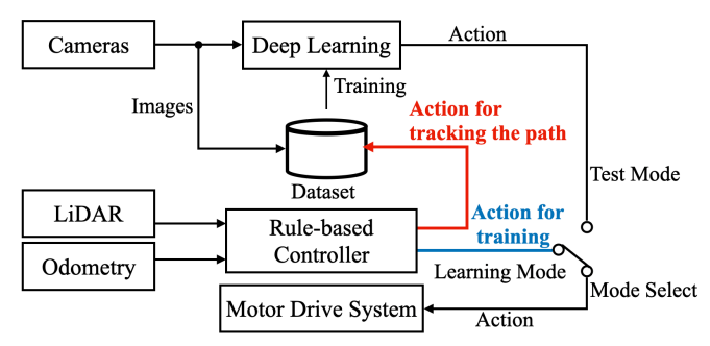
\includegraphics[width=100mm]{images/pdf/okada/method_sys.pdf}
   \caption[Structure of the Okada and others proposed system]{Structure of the Okada and others proposed system(Quoted from\cite{okada2020})}
   \label{fig:okada_sys}
\end{figure}
訓練時には,ROS の navigation パッケージを使用して,設定した経路を追従する.
ロボットの並進速度は0.2m/sに固定する.
その際,ロボットに取り付けたカメラから取得したRGB画像とルールベース制御器が出力するヨー方向の角速度をペアにして,0.2秒の周期でデータセットに追加する.
収集には3台のカメラを使用することで,データの多様性を高めるとともに過学習を防ぐ効果を狙っている.
また,左右のカメラ画像に対するヨー方向の角速度には経路復帰を補助するためのオフセット(\(\pm 0.2\)rad/s)を加える.

\figref{fig:okada_net}に岡田らの従来手法における学習器のネットワーク構造を示す.
% 学習器は入力をRGB画像データ,出力をロボットのヨー方向の角速度としている.
ネットワークは,入力層 1,畳み込み層 3,全結合層 2,出力層 1 の全7層で構成される.
データセットからはバッチサイズ8で教師データを抽出し,end-to-end学習を行う.

\begin{figure}[htbp]
    \centering
     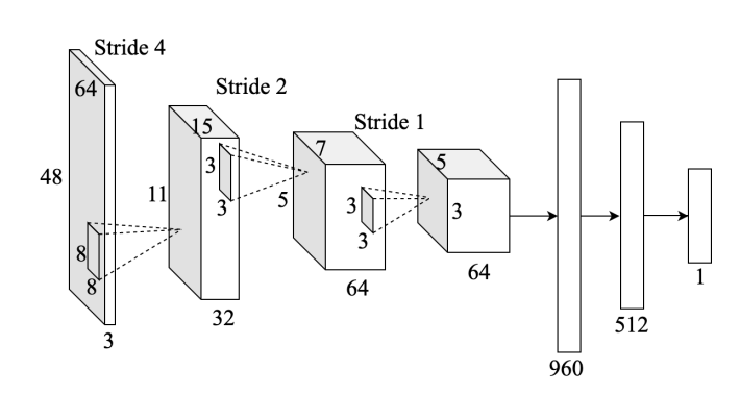
\includegraphics[width=100mm]{images/pdf/okada/network.pdf}
     \caption[Structure of the network used in the method of Okada and others]{Structure of the network used in the method of Okada and others(Quoted from \cite{okada2020})}
     \label{fig:okada_net}
\end{figure}

学習器の訓練後は,中央のカメラから得たRGB画像を入力とし,出力されるヨー方向の角速度を用いて経路を追従する.
この手法は実ロボットを用いて有効性が調査されており,\figref{fig:cource}に示す学習した経路を,画像のみを入力とした学習器の出力で自律移動できることが確認されている.

\begin{figure}[htbp]
  \centering
   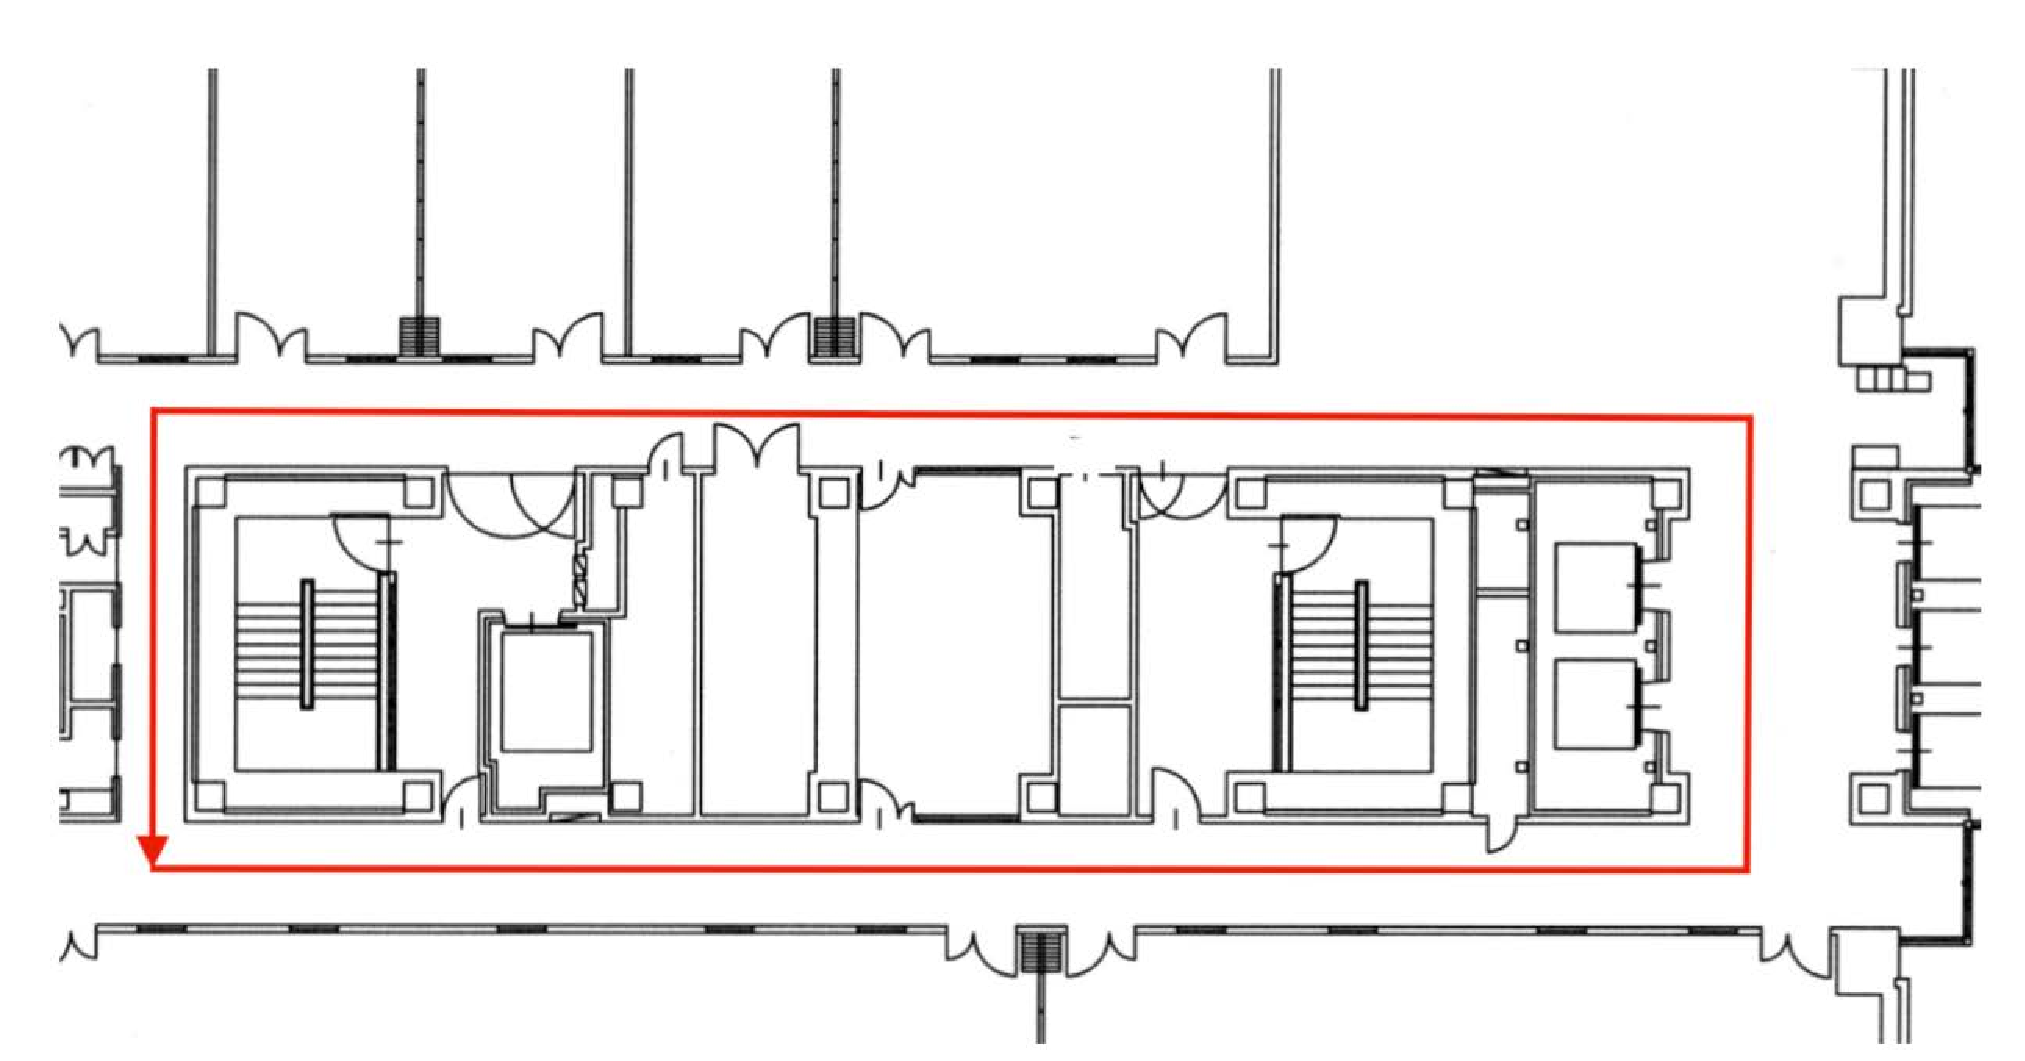
\includegraphics[width=80mm]{images/pdf/okada/cource.pdf}
   \caption{Target path used in the experiment(Quoted from \cite{okada2020})}
   \label{fig:cource}
\end{figure}
